% F081: f(x)=x^3-3x+1 has three distinct zeros; f' has two zeros.
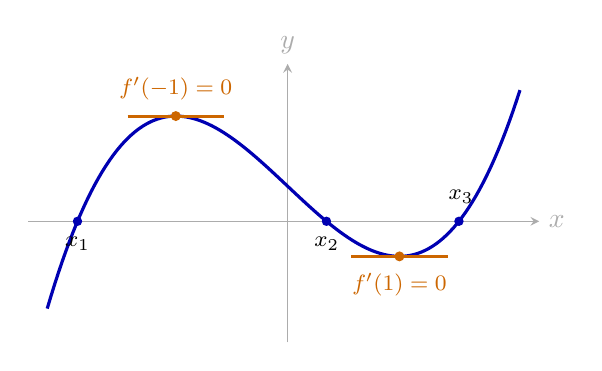
\begin{tikzpicture}[x=1.42cm,y=1.35cm,>=stealth]
  \draw[->,gray!65] (-2.32,0)--(2.25,0) node[right] {$x$};
  \draw[->,gray!65] (0,-1.14)--(0,1.48) node[above] {$y$};
  \draw[line width=1.15pt,blue!70!black,domain=-2.15:2.08,samples=130]
    plot (\x,{0.33*(\x*\x*\x-3*\x+1)});
  \foreach \r in {-1.879385,0.347296,1.532089} {
    \fill[blue!70!black] (\r,0) circle (1.7pt);
  }
  \draw[orange!80!black,line width=1.1pt] (-1.43,0.99)--(-0.57,0.99);
  \draw[orange!80!black,line width=1.1pt] (0.57,-0.33)--(1.43,-0.33);
  \fill[orange!80!black] (-1,0.99) circle (1.8pt) (1,-0.33) circle (1.8pt);
  \node[above,font=\footnotesize,orange!80!black] at (-1,1.05) {$f'(-1)=0$};
  \node[below,font=\footnotesize,orange!80!black] at (1,-0.4) {$f'(1)=0$};
  \node[below,font=\footnotesize] at (-1.88,-0.06) {$x_1$};
  \node[below,font=\footnotesize] at (0.35,-0.06) {$x_2$};
  \node[above,font=\footnotesize] at (1.55,0.08) {$x_3$};
\end{tikzpicture}
